\section{Downstream Tasks}
\label{sec:tasks}

We further evaluate the benefits of incorporating AR autoencoders into two downstream tasks: style transfer and image denoising. To assess the benefits of AR autoencoders, in each task, we simply replace the standard autoencoders by the AR versions without incorporating any additional task-specific priors or tuning. Despite not tailoring our architecture to each scenario, it obtains on-par or better results than well-established methods. Refer to \secref{sec:supp_additional} and \secref{sec:supp_proposed_method} for more results and full implementation details.

\subsection{Style Transfer via Robust Feature Alignment}
\begin{table}[t]
\centering
\begin{center}
\vspace{0.2 cm}
\caption{\label{tab:style_quantitative}Universal Style Transfer. Our AR AlexNet autoencoder outperforms both its standard counterpart and the original VGG-19 model in terms of Gram loss, the latter using more layers, larger feature maps and feature blending.}
\vspace{0.1 cm}
\resizebox{0.75\textwidth}{!}{%
\begin{tabular}{c|c|c|c|c|c}
\specialrule{.15em}{.05em}{.05em} 
\makecell{Encoder} & \makecell{Stylization\\Levels} & \makecell{Smallest\\Feature Map} & \makecell{Feature\\Blending} & \makecell{Gram Loss$\downarrow$\\$(x_{cs}, x_{s})$} & \makecell{SSIM$\uparrow$\\$(x_{cs}, x_{c})$}\\
\hline
\makecell{Standard AlexNet} & $3$ & $6\times6\times256$ & \xmark & $1.694$ & $0.226$\\\hline
\makecell{AR AlexNet (ours)} & $3$ & $6\times6\times256$ & \xmark & $\mathbf{1.186}$ & $\mathbf{0.259}$\\
\hline\hline
\makecell{VGG-19 \cite{simonyan_2014_very}} & $5$ & $14\times14\times512$ & \cmark & ${1.223}$ & ${0.459}$\\
\specialrule{.15em}{.05em}{.05em} 
\end{tabular}}
\end{center}
\vspace{-0.5 cm}
\end{table}

\begin{figure}[t]
\begin{minipage}{0.1\textwidth}
\centering\textbf{\colorbox{white}{\scalebox{.8}{Refs}}}
\end{minipage}\begin{minipage}[t]{0.2\textwidth}
\centering \textbf{\colorbox{white}{\scalebox{.8}{Standard}}}
\end{minipage}\begin{minipage}[t]{0.21\textwidth}
\centering \textbf{\colorbox{white}{\scalebox{.8}{AR (ours)}}}
\end{minipage}\begin{minipage}[t]{0.1\textwidth}
\centering\textbf{\colorbox{white}{\scalebox{.8}{Refs}}}
\end{minipage}\begin{minipage}[t]{0.2\textwidth}
\centering \textbf{\colorbox{white}{\scalebox{.8}{Standard}}}
\end{minipage}\begin{minipage}[t]{0.2\textwidth}
\centering \textbf{\colorbox{white}{\scalebox{.8}{AR (ours)}}}
\end{minipage}

\vspace{-0.1 cm}
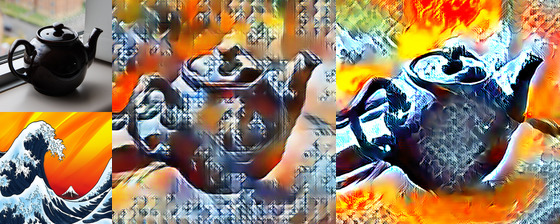
\includegraphics[width=0.5\textwidth]{figs/st/st_tile05.jpg}
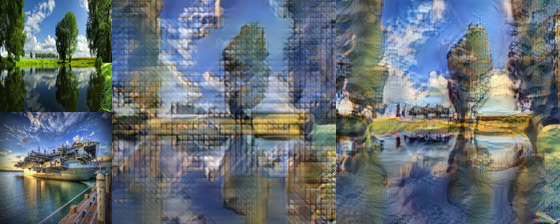
\includegraphics[width=0.5\textwidth]{figs/st/st_tile03.jpg}

\caption{\label{fig:style01}Universal Style Transfer: By inverting AR features, our autoencoder improves both content and style preservation, obtaining a better image stylization.}
\vspace{-0.7 cm}
\end{figure}

Motivated by the perceptual properties of AR features \cite{engstrom_2019_adversarial}, we analyze their impact on style transfer using our AR AlexNet autoencoder as backbone and measure their improvement in both structure and texture preservation.

\textbf{Experimental Setup.} Stylization is evaluated on $75$ random content images and $100$ random style images, leading to $7,500$ image pairs. Content and style preservation is evaluated via the SSIM between content and stylized images and the VGG-19 Gram loss between style and stylized images, respectively. \layer{Conv1} and \layer{conv2} models use nearest neighbor interpolation instead of transposed convolution layers to improve reconstruction and avoid checkerboard effects, while the \layer{conv5} model remains unaltered. We also include results using Universal Style Transfer's (UST) official implementation, using a VGG-19 backbone.

\textbf{Results.} Our AR autoencoder improves both texture and structure preservation over its standard version (\tabref{tab:style_quantitative}). Stylization via AR features removes artifacts in flat areas, reducing blurry outputs and degraded structure (\figref{fig:style01}). Besides, our AR model gets a lower Gram loss with respect to UST. This implies that, despite matching less feature maps than the VGG-19 model (three instead of five), stylizing via our AR AlexNet autoencoder better preserves the style.

As expected, UST obtains a better SSIM since VGG-19 has more complexity and uses less contracted feature maps than our AlexNet model (e.g. $14 \times 14 \times 512$ vs. $6 \times 6 \times 256$). Also, UST \textit{blends} stylized and content features to better preserve shapes. Overall, a comparison between our AR model and UST shows a tradeoff between content and style preservation.

\subsection{Image Denoising via AR Autoencoder}
Similarly to the robustness imposed by regularized autoencoders \cite{vincent_2010_stacked,rifai2011contractive,kingma_2013_auto}, we harness the manifold learned by AR models to obtain noise-free reconstructions. We evaluate our AR AlexNet denoising model and compare its restoration properties with alternative learn-based methods.
\begin{table}[t]
\vspace{0.3 cm}
\small
\def\arraystretch{1.25}
\setlength\tabcolsep{4pt}
\caption{\label{tab:denoising}Image denoising $(\sigma= \frac{50}{255})$: Our AR denoiser outperforms its standard version on multiple datasets. On the largest one (CBSD68), it also outperforms alternative learn-based techniques. On smaller sets (Kodak24, McMaster), it improves in SSIM and gets comparable PSNR and LPIPS performance.}
\vspace{-0.2 cm}
\begin{center}
\resizebox{\columnwidth}{!}{
\begin{tabular}{c|c|c|c|c|c|c|c|c|c}
\specialrule{.15em}{.05em}{.05em} 
& PSNR (dB)$\uparrow$ & SSIM$\uparrow$ & LPIPS$\downarrow$ & PSNR (dB)$\uparrow$ & SSIM$\uparrow$ & LPIPS$\downarrow$ & PSNR (dB)$\uparrow$ & SSIM$\uparrow$ & LPIPS$\downarrow$\\
\hline
Encoder & \multicolumn{3}{c|}{CBSD68} & \multicolumn{3}{c|}{Kodak24} & \multicolumn{3}{c}{McMaster}\\
\hline
\makecell{TNRD \cite{chen_2016_trainable}} & $24.75$ & $0.662$ & $0.445$ & $25.994$ & $0.695$ & $0.461$ & $25.01$ & $0.66$ & $\mathbf{0.387}$\\
\makecell{MLP \cite{burger_2012_image}} & $25.184$ & $0.663$ & $0.46$ & \makecell{$\mathbf{26.31}$} & $0.691$ & $0.478$ & \makecell{$\mathbf{26.039}$} & \makecell{$\mathbf{0.693}$} & \makecell{$0.402$}\\
\makecell{Standard} & \makecell{$22.6297$} & \makecell{$0.6178$} & \makecell{$0.567$} & \makecell{$23.1868$} & \makecell{$0.6001$} & \makecell{$0.4968$} & \makecell{$23.1493$} & \makecell{$0.6072$} & \makecell{$0.4458$}\\
\makecell{AR (ours)} & \makecell{$\mathbf{25.258}$} & \makecell{$\mathbf{0.7095}$} & \makecell{$\mathbf{0.4043}$} & \makecell{$25.4946$} & \makecell{$\mathbf{0.701}$} & \makecell{$\mathbf{0.447}$} & \makecell{$25.3527$}& \makecell{$0.6914$} & \makecell{$0.3965$}\\
\specialrule{.15em}{.05em}{.05em} 
\end{tabular}
}
\end{center}
\vspace{-0.7 cm}
\end{table}

\begin{figure}[t]
\begin{minipage}{0.25\textwidth}
\centering\textbf{\colorbox{white}{\scalebox{.8}{Ground-truth}}}
\end{minipage}\begin{minipage}[t]{0.25\textwidth}
\centering \textbf{\colorbox{white}{\scalebox{.8}{Observation}}}
\end{minipage}\begin{minipage}[t]{0.25\textwidth}
\centering \textbf{\colorbox{white}{\scalebox{.8}{Standard}}}
\end{minipage}\begin{minipage}[t]{0.25\textwidth}
\centering\textbf{\colorbox{white}{\scalebox{.8}{AR (ours)}}}
\end{minipage}

\vspace{-0.05 cm}
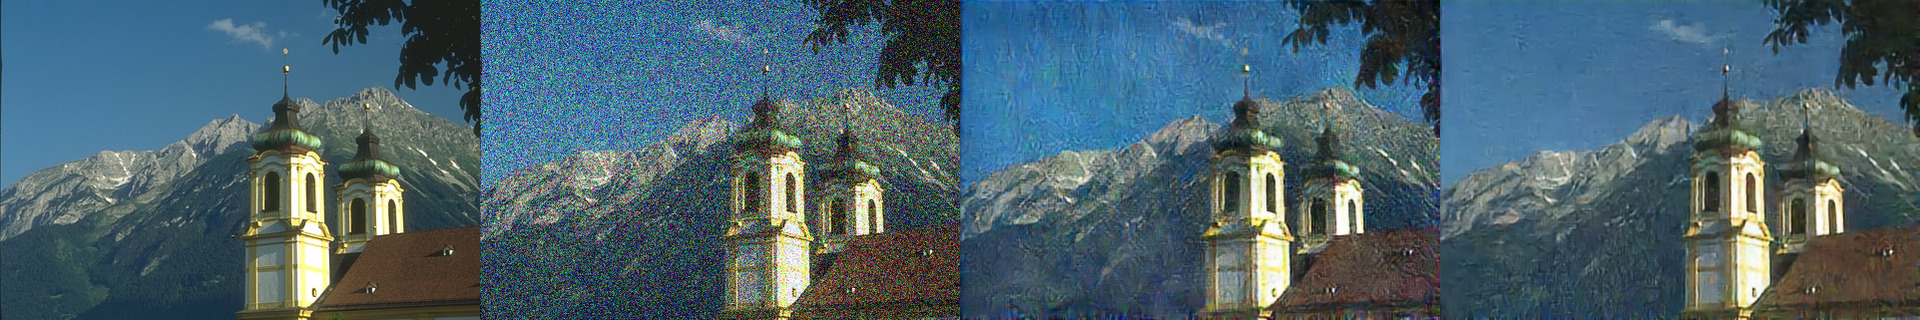
\includegraphics[width=1\textwidth]{figs/denoising/cbsd68_tile20.jpg}

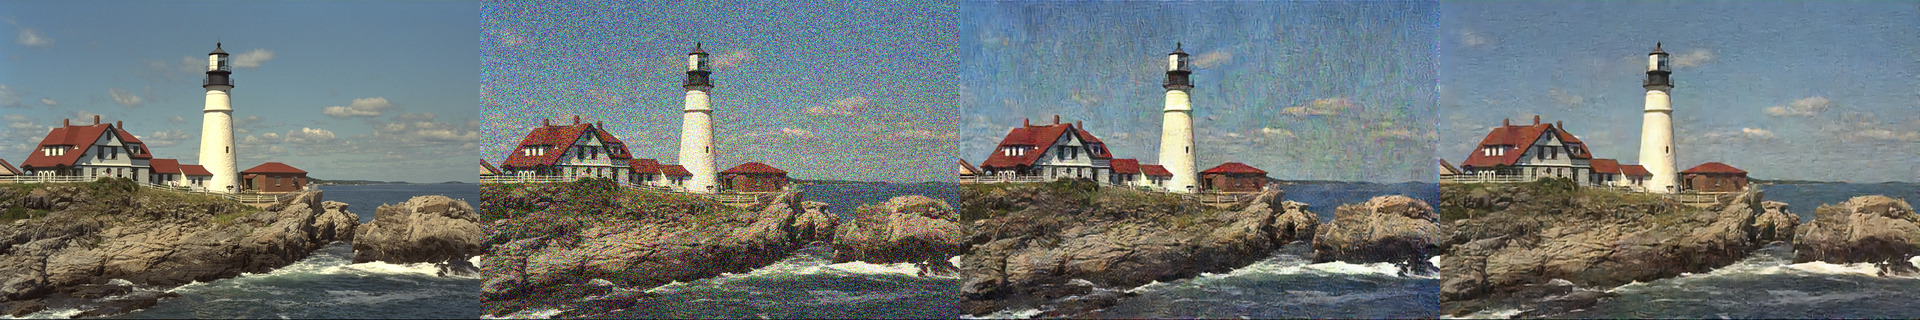
\includegraphics[width=1\textwidth]{figs/denoising/kodak24_tile20.jpg}

\caption{\label{fig:denoising}Image denoising $(\sigma= \frac{50}{255})$: While inverting standard features introduces artifacts and degrades color, limiting their use for restoration tasks, our AR denoiser reduces the artifacts and better preserves the original texture.}
\vspace{-0.5 cm}
\end{figure}


\textbf{Experimental Setup.} Our image denoising model consists of an AR autoencoder equipped with skip connections in \layer{conv1}, \layer{conv2} and \layer{conv5} layers to better preserve image details. Skip connections follow the Wavelet Pooling approach \cite{yoo_2019_photorealistic}. Generators are trained on ImageNet via pixel and feature losses.

Accuracy is evaluated on the Kodak24, McMaster \cite{zhang_2011_color} and Color Berkeley Segmentation Dataset 68 (CBSD68) \cite{MartinFTM01} for clipped additive Gaussian noise ($\sigma=50/255$). We compare our AR model against two learn-based methods, Trainable Nonlinear Reaction Diffusion (TNRD) \cite{chen_2016_trainable} and Multi Layer Perceptron-based model (MLP) \cite{burger_2012_image}, often included in real-noise denoising benchmarks \cite{anwar_2019_real,guo_2019_toward}.

\textbf{Results.}  Our AR model improves over its standard version in all metrics across all datasets (\tabref{tab:denoising}). While standard predictions include color distorsions and texture artifacts, AR predictions show a better texture preservation and significantly reduce the distorsions introduced by the denoising process (\figref{fig:denoising}).

Our AR model obtains the best PSNR, SSIM and LPIPS scores on CBSD68, the most diverse of all datasets. While it is outperformed in PSNR by MLP in the two remaining datasets, it improves in SSIM and LPIPS, getting best or second best performance. For the McMaster dataset, SSIM and LPIPS values obtained by our model are slightly below the best values. Overall, our model consistently preserves the perceptual and structural similarity across all datasets, showing competitive results with alternative data-driven approaches.
